\documentclass[10pt,a4paper]{article}
\usepackage{tikz}
\usetikzlibrary{through}
\begin{document}
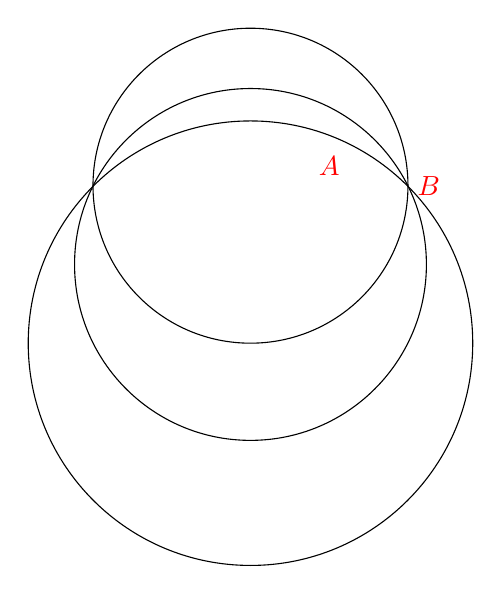
\begin{tikzpicture}
\coordinate [label=above:\textcolor{red}{$A$}] (A) at (1,2);
\coordinate [label=right:\textcolor{red}{$B$}] (B) at (2,2);
% Works
\node [draw] at (0,0) [circle through={(B)}] {};
\node [draw] at (0,1) [circle through=(B)] {};
\node [draw] at (0,2) [circle through={(2,2)}] {};
% Doesn't work
%\node [draw] at (A) [circle through=(2,2)] {};
\end{tikzpicture}
\end{document}